\section{Full-Body-Tracking}
\label{sec:full-body-tracking}
\setauthor{Quirin Ecker}

Das Full-Body-Tracking wurde mit einem kostenpflichtigen Plugin namens Final IK implementiert.
Dieses Plugin ist für die Arbeit gratis zur Verfügung gestellt worden.

Bevor Full-Body-Tracking benutzt werden kann, muss das Tracking erstmals kalibriert werden.
In BeamVR funktioniert die Kalibration des Full-Body-Trackings mit dem Trackpad auf dem Controller.
Diese Taste ist in Abb.~\ref{fig:vive-controller-trackpad} zu sehen.
Die Taste für das Kalibrieren wird in der Inbetriebnahme, welche in Abschnitt~\ref{ch:commisioning} beschrieben wird, benutzt.

Standardmäßig wird in FinalIK das Full Body Tracking mit der Taste C kalibriert.
Damit die Kalibration auch in VR erfolgen kann, ist eine Taste für das kalibrieren auch auf dem Controller reserviert.
Wie bereits beschrieben ist diese Taste das Trackpad auf dem Controller.

Um das Kalibrieren auf eine andere Taste zu stellen, werden die Daten für das Full-Body-Tracking an die eine Script-Komponente übergeben.
Diese Script-Komponente horcht auf Tastenbetätigungen des Trackpad.
Sobald die Taste gedrückt wird, wird die statische Funktion \emph{Calibrate()} der Klasse \emph{Calibrate()} mit den übergebenen Daten aufgerufen.

Um zu checken, ob die Taste gedrückt wird, benützen wir das SteamVR Plugin.
In Listing~\ref{lst:defining-control-objects} werden die Objekte für das Kontrollieren der Tasten zugewiesen.
Mit diesen Objekten kann mithilfe der Update-Methode auf einen Tastendruck gehorcht werden.
Das Horchen auf diese Taste ist in Listing~\ref{lst:checking-for-input} ersichtlich.
In diesem Fall muss auf die Taste beider Controller gehorcht werden, weshalb hier auf zwei Tasten gehorcht wird.

\begin{lstlisting}[language={[Sharp]C},label={lst:defining-control-objects}, caption={Zuweisung der Kontroll Objekt}]{Zuweisung der Kontroll Objekte}
private readonly SteamVR_Action_Boolean _inputAction = SteamVR_Actions.default_Teleport;
private const SteamVR_Input_Sources RightController = SteamVR_Input_Sources.RightHand;
private const SteamVR_Input_Sources LeftController = SteamVR_Input_Sources.LeftHand;
\end{lstlisting}

\begin{lstlisting}[language={[Sharp]C},label={lst:checking-for-input}, caption={Auf Nutzerinput warten}]{Auf Nutzerinput warten}
private void Update()
{
    if (_inputAction.GetStateDown(RightController) || _inputAction.GetStateDown(LeftController))
    {
        // Calibrate();
        ...
    }
}
\end{lstlisting}

Wie bereits beschrieben werden die Daten der Script-Komponente übergeben.
Das Object welches diese Daten hält ist von dem Typen \emph{VRIKCalibrationController}.
Dieses wird schlussendlich wie in Listing~\ref{lst:vrik-calibration} verwendet.

\begin{lstlisting}[language={[Sharp]C},label={lst:vrik-calibration}, caption={Kalibrierung}]{Kalibrierung}
_calibrationControllerObject.data = VRIKCalibrator.Calibrate(
    _calibrationControllerObject.ik,
    _calibrationControllerObject.settings,
    _calibrationControllerObject.headTracker,
    _calibrationControllerObject.bodyTracker,
    _calibrationControllerObject.leftHandTracker,
    _calibrationControllerObject.rightHandTracker,
    _calibrationControllerObject.leftFootTracker,
    _calibrationControllerObject.rightFootTracker
);
\end{lstlisting}

\section{Schwerkraft}
\label{sec:gravity}

Damit die Applikation eine gewisse Spannung erhält, gibt es auch die Möglichkeit von dem Balken runterzufallen.
Dies sollte passieren, sobald die Person auch in der physischen Realität von dem Balken fällt.
Folgend ist die Bedingung für einen Fall beschrieben.

\subsection{Bedienung}\label{subsec:bedienung}

Bei der implementierung des Fallens muss es bestimmte Bedienungen geben, bei denen die Spielerin oder der Spieler herunterfallen soll.
Die erste Bedienung ist, dass die Benutzerin oder der Benutzer sich über dem Abgrund befindet.
Befindet sich die Person noch auf dem Haus, steht sie zwar nicht auf dem Balken, sollte aber trotzdem nicht herunterfallen.

Die zweite Bedingung ist, ab wann eine Person, welche sich über dem Abgrund befindet, von dem Balken herunterfliegt.
Grundsätzlich fliegt die Benutzerin oder der Benutzer von dem Balken, wenn diese oder dieser das Gleichgewicht verliert.
Der einfachheitshalber wurde keine Bedingung anhand des Gleichgewichtes implementiert.

Schlussendlich musste die Entscheidung getroffen werden, ob die Benutzerin oder der Benutzer bereits bei einem Fuß der bei zwei Füßen am Boden herunterfliegt.
In der BeamVR Applikation ist die Entscheidung auf die Bedingung mit einem Fuß auf dem Boden gefallen.
Somit fällt die Benutzerin oder der Benutzer von dem Balken herunter, sobald ein Fuß der Person auf dem Boden ankommt.

\subsection{Funktionsweise}\label{subsec:funktionsweise}

\begin{figure}
    \centering
    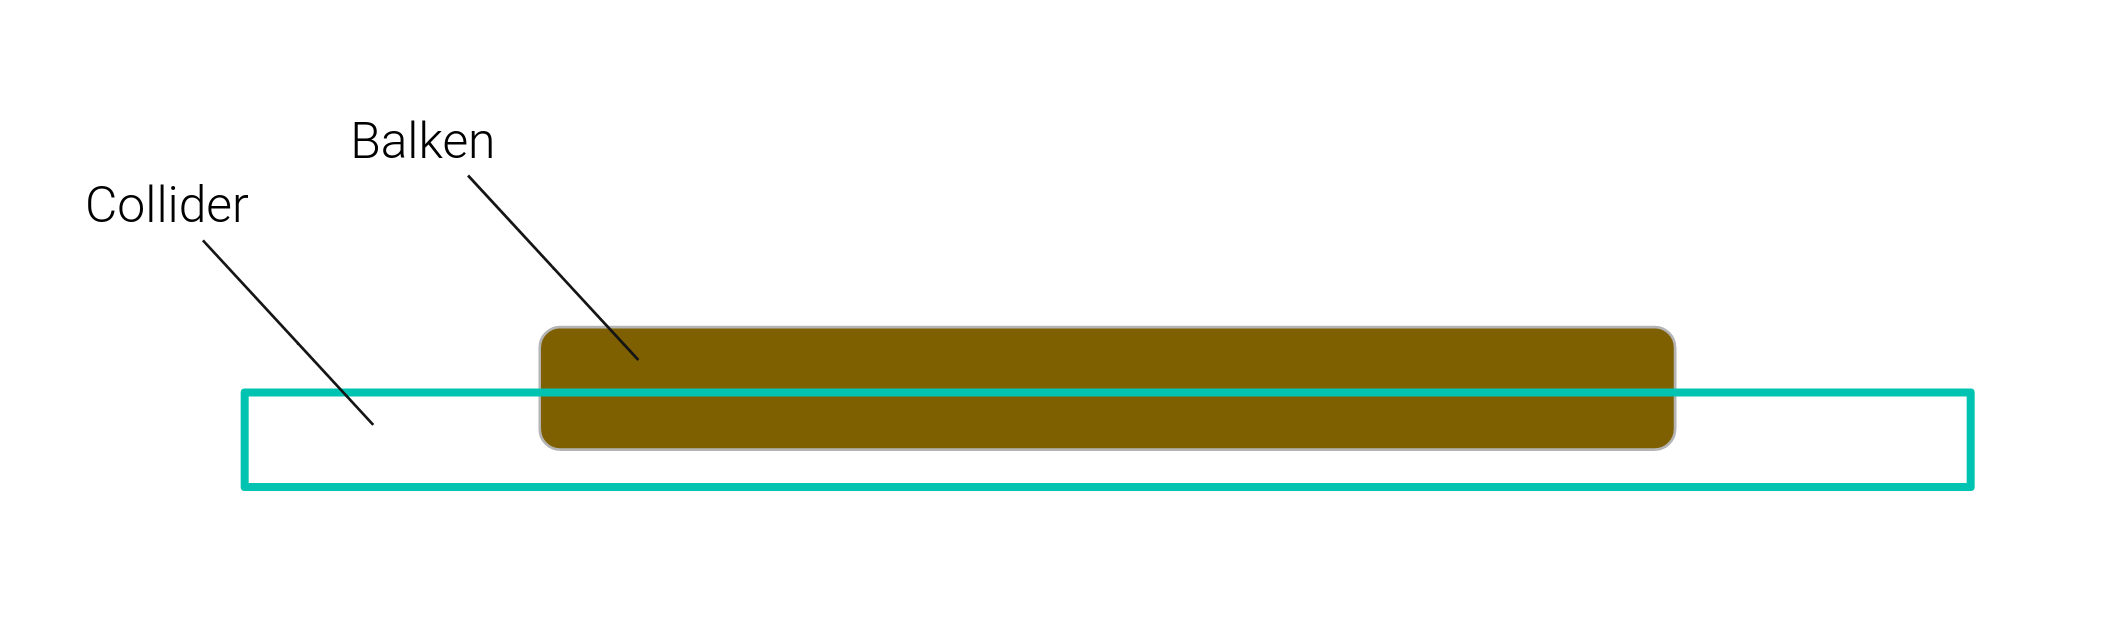
\includegraphics[scale=0.2]{pics/gravitation_collider}
    \caption{Schwerkraft Collider}
    \label{fig:gravitation-collider}
\end{figure}


Um zu checken, ob ein Fuß sich auf dem Boden befindet wurde ein Collider unter den Balken in der Höhe des Bodens platziert.
Diesen Collider ist eine unsichtbare Box, die nur für die Überprüfung möglicher Kollision existiert.
In Abb.~\ref{fig:gravitation-collider} ist diese Anordnung visualisiert.

Die Höhe des Bodens wird durch das SteamVR Setup ermittelt.
Hier werden die Kontroller auf den Boden gelegt und in dem Setup auf Kalibrieren gedrückt, um die Höhe des Bodens zu ermitteln.
Dies funktioniert anhand der getrackten Controller.
Weitere Informationen über das SteamVR Setup können in Abschnitt~\ref{sec:steam-vr-setup} gefunden werden.

Kollidiert einer der Füße mit dem Collider, wird die gesamte VR Fläche mit einer Beschleunigung von 9.81 m/s nach unten bewegt.
Kurz bevor die Fläche auf dem Boden aufkommt, wird in eine ander Szene gewechselt.

Um die Möglichkeit zu verhindern, dass der Kopf durch das Haus fliegt, da nur die füße sich auf dem Boden befinden und der Kopf immer noch über dem Haus wurde ein weiterer Check eingebaut.
Dieser Check beinhaltet, dass das Headset sich über dem Collider befinden muss, damit die Spielerin oder der Spieler runterfliegt.
Befindet sich das Headset noch über dem Haus kann der Spieler oder die Spielerin nicht von dem Haus fliegen.

\section{Verkehrssystem}
\label{sec:traffic-system}
\setauthor{Florian Beckerle}
In der Stadt von BeamVR ist auf den Straßen einiges los, dass wurde mithilfe eines neuen Verkehrssystems umgesetzt.
Die Straßen sind mit, f\"ur den Spieler unsichtbaren, Objekten versehen, die den Verkehr regeln.

\textbf{Car Signals}
Damit die Fahrzeuge in BeamVR wissen wo und vor allem wie sie auf den Straßen navigieren k\"onnen, wurde das Car Signal System entwickelt.
Die Car Signals gibt es in zwei verschiedenen Versionen, f\"ur die linke Straßenseite wurden gr\"une und f\"ur die rechte Seite wurden rote Signale erstellt.
Die Signale funktionieren wie Checkpoints.
Jedes Auto wird, nachdem es initialisiert wurde, von einem zum n\"achsten fahren.
Jeder dieser Checkpoints verweist auf den nächsten, wie in einer Liste, daher weiß jedes Fahrzeug, wo die momentane Zielposition ist.~\ref{fig:trafficsystem_next_signal_reference}
Endpunkte sind spezielle Signale, welche auf keinen nachfolgenden Punkt mehr verweisen.
Erreicht ein Auto ein solchen Punkt, hat es das Ziel erreicht.

An Kreuzungen befinden sich mehrere dieser Car Signals, damit die Fahrzeuge auf der richtigen Spur bleiben und die Verkehrsregeln befolgen.
Die gr\"unen Linien zeigen die m\"oglichen Routen, die das Auto fahren kann.
Die Pfeile visualisieren, in welche Richtung gefahren werden kann, siehe Abb.~\ref{fig:trafficsystem_crossroads}.


\begin{figure}
    \centering
    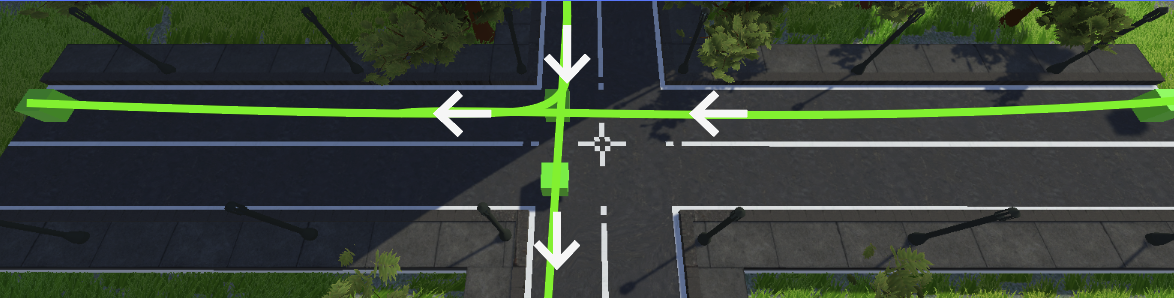
\includegraphics[scale=0.5]{pics/trafficsystem_carsignal_crossroads}
    \caption{Traffic System - Crossroads}
    \label{fig:trafficsystem_crossroads}
\end{figure}

\begin{figure}
    \centering
    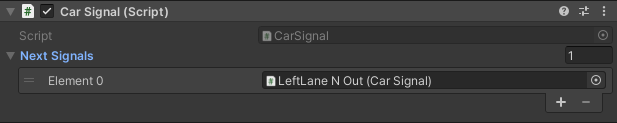
\includegraphics[scale=0.7]{pics/trafficsystem_carsignal_signal_reference}
    \caption{Traffic System - Next Signal Reference}
    \label{fig:trafficsystem_next_signal_reference}
\end{figure}


\textbf{Car Spawn Points}
Car Spawn Points sind blau dargestellte Punkte, an denen Fahrzeuge nach dem Laden der Szene initialisiert werden, siehe Abb.~\ref{fig:trafficsystem_car_spawn_points}.
Falls ein Auto einen Car Signal, welcher ein Endpunkt ist, erreicht, wird es nach einem kurzen Delay an einem Respawn Point wieder erscheinen.
Diese Punkte verweisen, \"ahnlich wie Car Signals, auf einen nachfolgenden Punkt, wo die Fahrzeuge hinfahren.

%% IN QUELLCODEVERZEICHNIS PACKEN!
\begin{lstlisting}{CarSpawnPoint.cs}
public class CarSpawnPoint : MonoBehaviour
{

    //Location where the car should go after respawning
    public CarSignal nextSignal;

    //Position of the Respawnpoint;
    public Vector3 position;

    public void Start(){
        position = transform.position;
    }

    public Vector3 GetPosition(){
        return position;
    }

    public CarSignal GetNextSignal(){
        return nextSignal;
    }

}
\end{lstlisting}

\begin{figure}
    \centering
    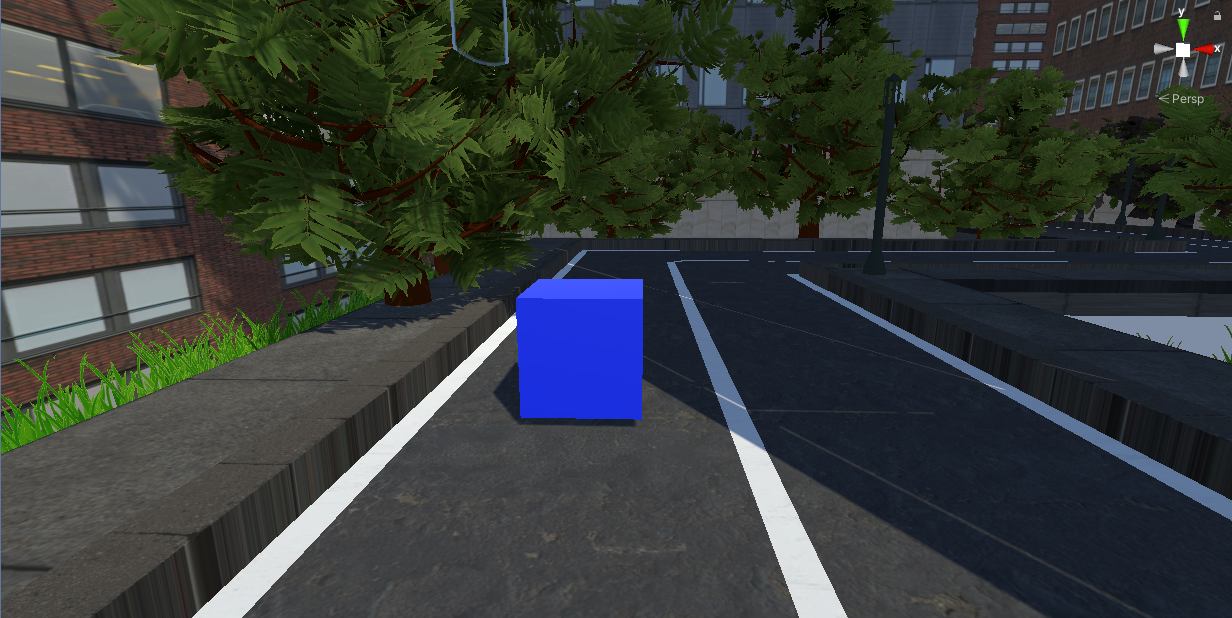
\includegraphics[scale=0.4]{pics/trafficsystem_respawn_point}
    \caption{Traffic System - Car Spawn Points}
    \label{fig:trafficsystem_car_spawn_points}
\end{figure}


\textbf{Car Manager}
Der Car Manager regelt die maximale Anzahl an Fahrzeugen die gleichzeitig auf den Straßen fahren k\"onnen.
Am Anfang werden n Fahrzeuge (n ist hierbei die maximale Anzahl an Autos) auf den Straßen initialisiert, indem ein zuf\"alliger Spawn Point ausgewählt wird.
\begin{lstlisting}{car_manager_respawncars}

public void SpawnCar(){
        CarSpawnPoint newCarSpawnPoint = GetRandomSpawnPoint();
        GameObject newCar = Instantiate(GetRandomCarModell(), newCarSpawnPoint.GetPosition(), newCarSpawnPoint.transform.rotation);
        newCar.GetComponent<CarBehaviour>().SetCarManager(this);
        CarBehaviour carBehaviour = newCar.GetComponent<CarBehaviour>();


        carBehaviour.curSignal = newCarSpawnPoint.GetNextSignal();
        carBehaviour.curPosition = newCarSpawnPoint.GetPosition();

        currentCars.Add(newCar);
    }
\end{lstlisting}

Weiters wird mithilfe der Funktion RespawnCars() ein Auto recycled, sobald es einen Endpunkt erreicht hat, indem der Manager die aktuelle Position und das n\"achste Ziel des Fahrzeuges neu setzt.
\begin{lstlisting}{car_manager_respawncars}
public void RespawnCars(GameObject finishedCar){
        CarBehaviour carBehaviour = finishedCar.GetComponent<CarBehaviour>();
        CarSpawnPoint newCarSpawnPoint = GetRandomSpawnPoint();
        carBehaviour.curSignal = newCarSpawnPoint.GetNextSignal();
        carBehaviour.curPosition = newCarSpawnPoint.GetPosition();
    }
\end{lstlisting}

\textbf{Car Behaviour}
Jedes Fahrzeug erh\"alt, nachdem es initialisiert wurde, eine zufällige ID mit folgendem Aufbau "Car[0-9]BeamVR[0-9]", damit diese im sp\"ateren Verlauf des Spieles besser identifiziert werden können.
In jedem Frame bewegt sich das Auto mithilfe der Vector3.MoveTowards() Funktion in Richtung dem Car Signal, welches als Ziel festgelegt wurde.
Wenn nun das momentane Ziel erreicht wurde, sucht das Gefährt in dem aktuellen Punkt die Referenz auf das nächste Signal und bewegt sich dorthin.

Um zu verhindern, dass mehrere Fahrzeuge ineinander fahren, kann das Auto mithilfe eines Raycasts erkennen, was sich in einer bestimmten Distance vor ihm befindet und im Notfall anhalten.

\begin{lstlisting}{car_behaviour_raycast}
...
RaycastHit hit;
         if (!Physics.Raycast(curPosition, transform.TransformDirection(Vector3.forward), out hit, carSeeingDist, layerMask))
        {
        ...
        }
...
\end{lstlisting}

\section{Beam Kalibration}
\label{sec:beam-calibration}
\setauthor{Quirin Ecker}

Das Kernthema dieser Arbeit ist, ein reales Objekt in die virtuelle Welt zu synchronisieren.
Im Falle unserer Arbeit ist dieses Objekt wie bereits beschrieben ein Balken.

Die Beam Kalibration ist für die Synchronisation des physischen und virtuellen Balkens zuständig.
In der Entwicklungsphase gab es mehrere Ansätze diese Synchronisation zu implementieren.
Hier ist zwischen Grundansätzen und Implementierungsansätze zu unterscheiden.
Im Zuge dieser Arbeit beschreibt ein Grundansatz die grundlegende Strategie das Problem zu lösen und ein Implementierungsansatz die Strategie einen Grundansatz zu lösen.

\subsection{Grundansätze}\label{subsec:grundansaetze}

Folgend werden zwei dieser Grundansätze beschrieben.

\subsubsection{Tracker Ansatz}

Der Initial-Ansatz dieser Arbeit war der \emph{Tracker Ansatz}.
Dieser Ansatz war eine Lösung mit den Vive Trackern.
In diesem Lösungsansatz würde ein Tracker in die Mitte des Balkens platziert werden.
Durch diesen Tracker und die Dimensionen des Balkens würde es in der Theorie möglich sein die Position und größe des Balkens zu berechnen.

Der Vorteil dieses Ansatzes wäre, dass der Balken während des Spielerlebnis verschiebbar ist, da die Position durch den Tracker aktualisiert werden kann.

Leider besitzt dieser Ansatz durch die Benutzung des Trackers einige Nachteile.
Einer dieser Nachteile ist, dass die Dimensionen des Balkens beim Initial Setup gemessen werden müssen.
Weiters muss der Tracker in der mitte des Balkens befestigt werden, da durch Änderungen der Position des Trackers auch Änderungen des virtuellen Balkens auftreten.
Bei keiner Befestigung kann der Tracker leicht verrutschen.
Schlussendlich muss auch die Mitte des Balkens ermittelt werde, um den Tracker dort zu platzieren.
Wenn die Ermittlung ungenau ist, wird es zu einer ungenauen Synchronisation führen.

\subsubsection{Marker Ansatz}

Für die BeamVR Applikation reicht es normal aus, dass die Skalierung, Position und Orientierung einmal vor dem Spielerlebnis ermittelt werden.
Das bedeutet, dass die dynamische Änderung der Position in den meisten Fällen vernachlässigt werden kann.

Bei dem Marker Ansatz werden keine zusätzlichen Geräte wie Tracker gebraucht.
Für das Kalibrieren des Balkens wird dabei einer der Controller verwendet

Im Prinzip wird bei diesem Ansatz der Controller verwendet, um die Ecken des Balkens zu markieren.
Diese Markierungen werden von der Applikation gespeichert und später in der Game-Szene verwendet, um den Balken richtig zu positionieren, skalieren und orientieren.
Da die Höhe durch das SteamVR Setup bekannt ist, müssen nur die oberen Ecken des Balkens.
Für mehr Informationen über das SteamVR Setup wird auf den Abschnitt~\ref{sec:steam-vr-setup}.

\begin{figure}
    \centering
    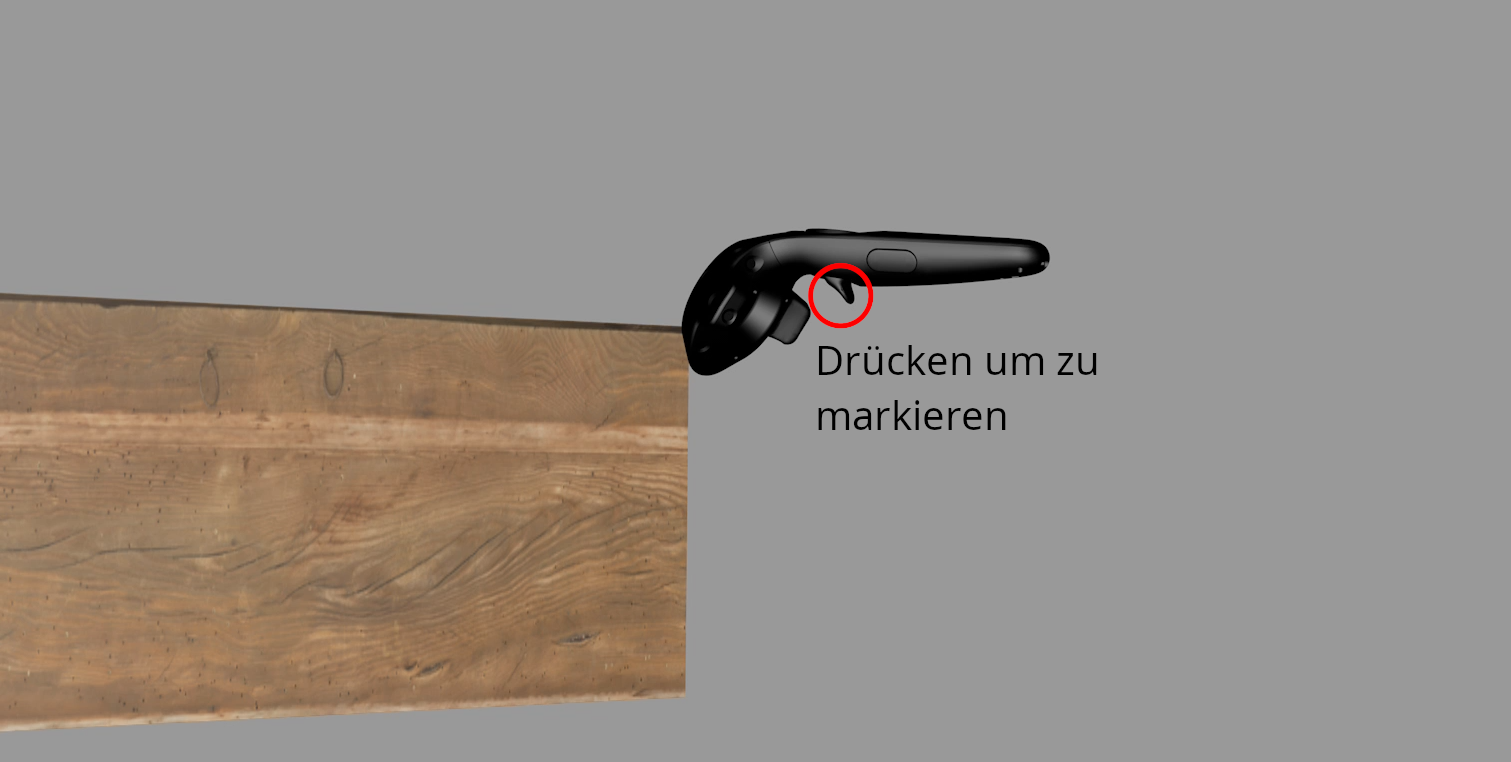
\includegraphics[scale=0.3]{pics/beam_mark}
    \caption{Markierung Einer Ecke des Balkens}
    \label{fig:beam-mark}
\end{figure}

Eine dieser Markierung wird folgendermaßen durchgeführt.
Der Ring am Ende des Controller muss an der gewünschten Ecke anstoßen.
Daraufhin wird der Trigger gedrückt, welcher sich an der unteren seite des Controller befindet.
In Abb.~\ref{fig:beam-mark} ist dieser Vorgang dargestellt.

\begin{figure}
    \centering
    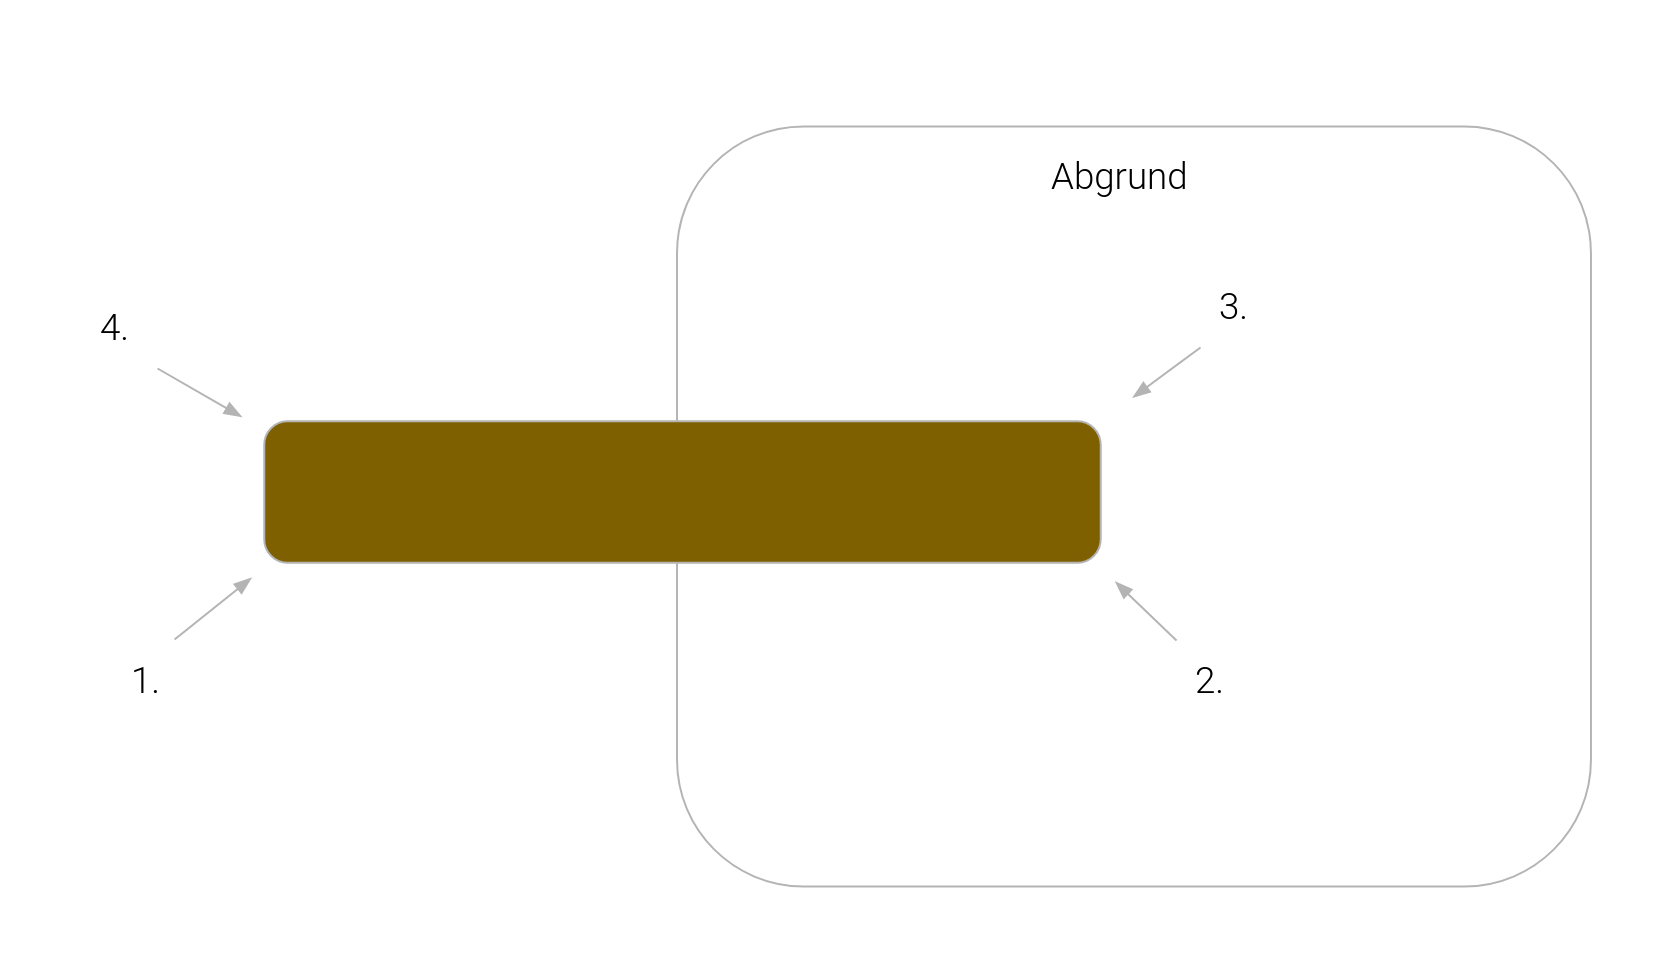
\includegraphics[scale=0.25]{pics/beam-marking-sequence}
    \caption{Reihenfolge der Markierungen}
    \label{fig:beam-marking-sequence}
\end{figure}

Insgesamt muss jede obere Ecke mit dem zuvor beschriebenen Vorgang markiert werden.
Für die Markierung jeder Ecke gibt es eine gewisse Reihenfolge.
Diese Reihenfolge ist von der BeamVR Applikation vordefiniert und von der Position des Abgrunds abhängig.
In Abb.~\ref{fig:beam-marking-sequence} ist die Reihenfolge ersichtlich.

Da die dynamische Positionsänderung während der Laufzeit in der BeamVR Applikation vernachlässigt werden kann wurde der Marker-Ansatz für die finale Applikation gewählt.

\subsection{Basisberechnungen}
\label{subsec:basisberechnungen}

\begin{figure}
    \centering
    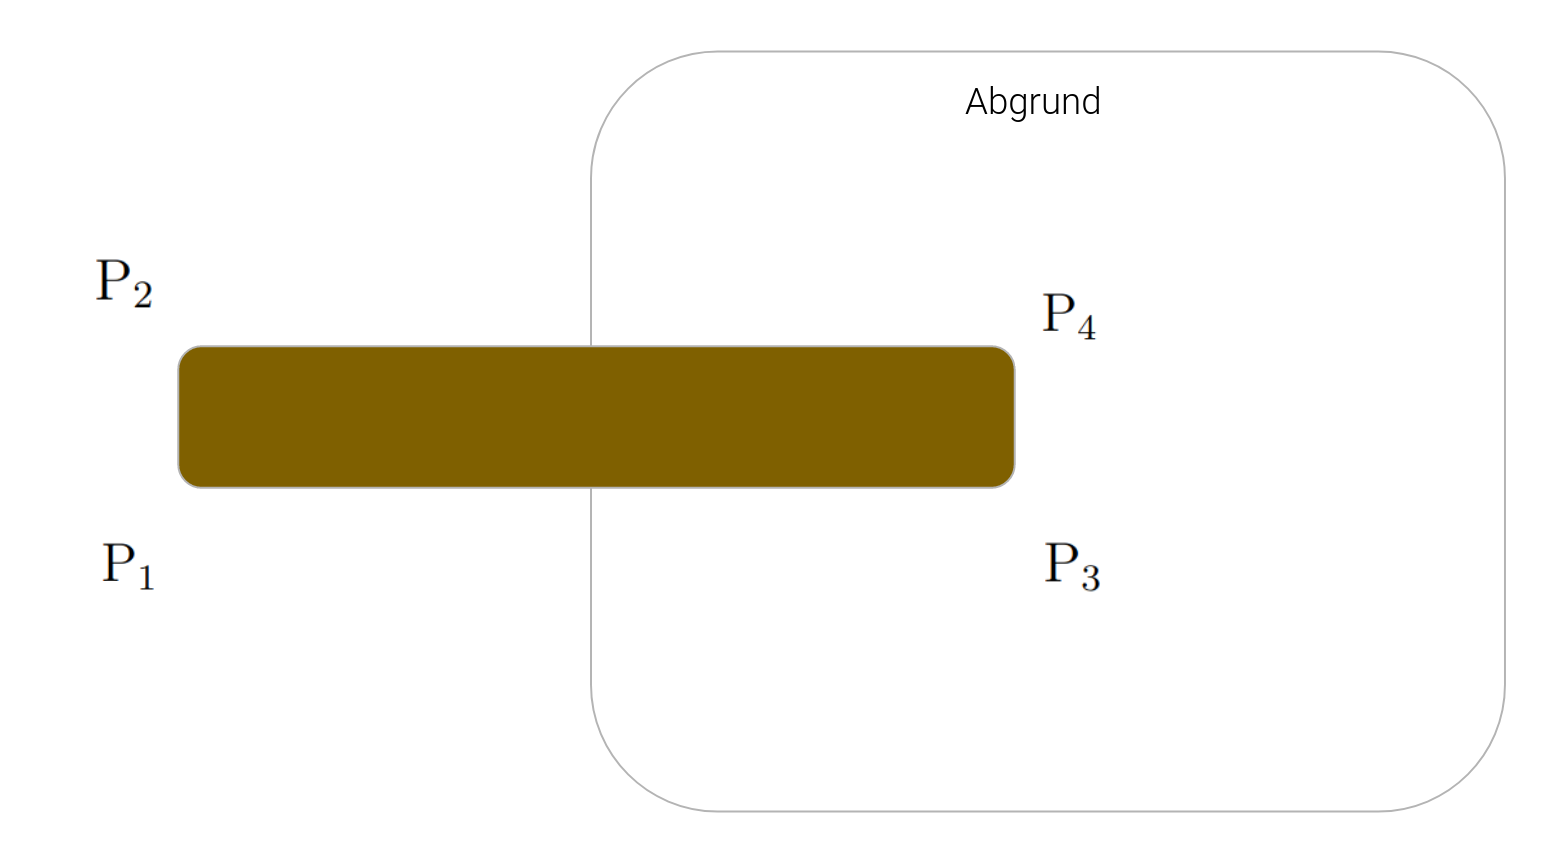
\includegraphics[scale=0.25]{pics/beam-point-labeling}
    \caption{Beschriftungen des Balkens}
    \label{fig:beam-point-labeling}
\end{figure}


Durch die Postionen der Ecken kann die Mitte des Balkens berechnet werden, da davon ausgegangen werden kann, dass der Balken ein Quader ist.
In Abb.~\ref{fig:beam-point-labeling} sind die Ecken der oberen Seite des Balken mit $P_{1}, P_{2}, P_{3}, P_{4}$ beschriftet.
Diese Punkte beschreiben die Reihenfolge, in der die Punkte der unteren seite $O_{1}, O_{2}, O_{3}, O_{4}$ und der oberen Seite $U_{1}, U_{2}, U_{3}, U_{4}$ angeordnet sind.
Alle restlichen Variablen können in der Tabelle~\ref{tab:variables} eingesehen werden.
Die Mitte der oberen Decke kann mit der folgenden Formeln berechnet werden.

\begin{table}[]
    \centering
    \begin{tabular}{|l|l|}
        \hline
        $O_{1}, O_{2}, O_{3}, O_{4}$ & Ecken der oberen Seite des Balkens                 \\ \hline
        $U_{1}, U_{2}, U_{3}, U_{4}$ & Ecken der unteren Seite des Balkens                \\ \hline
        $h$                          & Höhe des Balkens                                   \\ \hline
        $w$                          & Breite des Balkens                                 \\ \hline
        $l$                          & Länge des Balkens                                  \\ \hline
        $M_{O}$                      & Mittelpunkt der oberen Seite des Balkens           \\ \hline
        $M_{U}$                      & Mittelpunkt der unteren Seite des Balkens          \\ \hline
        $M$                          & Mittelpunkt des Balkens                            \\ \hline
        $D_{OU}$                     & Diagonale der unteren und oberen Seite des Balkens \\ \hline
        $V_{MU}$                     & Mittelpunkt des VR Raums am Boden                  \\ \hline
    \end{tabular}
    \caption{Basisvariablen}
    \label{tab:variables}
\end{table}

\pagebreak

$\vec{D_{OU}} = O_{4} - O_{1}$

$M_{OU} = O_{1} +  \frac{\vec{D_{OU}}}{2} $

$\vec{h} = (O_{4} - VM_{U}) \cdot \begin{bmatrix} 0 \\ 0 \\ 1  \end{bmatrix}$

$M = M_{OU} + \frac{\vec{h}}{2}$

Für die Skalierung des Balkens werden noch die Dimensionen des Balkens gebraucht.
Diese Dimensionen werden einfach mit dem Betrag der Vektoren folgendermaßen berechnet.

$h = |\vec{h}|$

$b = |\vec{O_{1}O_{3}}|$

$w = |\vec{O_{2}O_{4}}|$

\subsection{Implementierungsansatz}
\label{subsec:implementierungsansatz}

Für den Marker Ansatz gibt es wiederum zwei verschiedene Implementierunsansätze.
Diese beinhalten:

\begin{itemize}
    \item Beam Transformation Ansatz
    \item Player Transformation Ansatz
\end{itemize}

\subsubsection{Beam Transformation Ansatz}

Der einfachere Ansatz ist der Beam Transformation Ansatz.
Bei diesem Ansatz wird der virtuelle Balken an den physischen Balken angepasst.

Durch die Basisberechnungen ist der Mittelpunkt des physischen Balkens bekannt.
Die standardmäßige Position des Ankers befindet sich in Unity in der Mitte des Elements~\cite{AM_APPS_2020}.
Somit müssen die Koordinaten des virtuellen Balkens zu den Koordinaten des Mittelpunktes von dem physischen Balken gesetzt werden.

In Unity kann die Position wie in Listing~\ref{lst:beam-transformation-position} gesetzt werden.
Dabei ist die Variable \emph{beam} das Transform Object des virtuellen Balkens und M der Mittelpunkt des physischen Balkens.


\begin{lstlisting}[language={[Sharp]C},label={lst:beam-transformation-position}, caption={Beam Positionstranformation}]{Beam Positionstranformation}
    beam.position = M;
\end{lstlisting}

Für die Skalierung-Anpassung kann die berechnete Höhe, Länge und Breite verwendet werden.
Die Skalierung wird in Unity wie in der Listing~\ref{lst:beam-transformation-scale} gesetzt.
Dabei ist die Variable \emph{beam} das Transform Objekt des virtuellen Balkens, \emph{l}  die Länge, \emph{h} die Höhe und \emph{w} die Breite.

\begin{lstlisting}[language={[Sharp]C},label={lst:beam-transformation-scale}, caption={Beam Skalierungstransformation}]{Beam Skalierungstransformation}
    beam.localScale = new Vector3(l, h, w);
\end{lstlisting}

Der Beam Transformation Ansatz ist der leichtere Implementierungsansatz.
Nachteil dieser Implementierung ist aber, dass große Differenzen zwischen des physischen und des virtuellen Balkens zu unrealistischen Positionen führen.
Damit der Balken trotzdem in einer realistischen Position bleibt, gibt es den zweiten Implementierungsansatz.

\subsubsection{Player Transformation Ansatz}

Anstatt den Balken eine neue Position zu geben wird bei dem Player Transformation Ansatz die Startposition der Spielerin oder des Spielers versetzt.
Somit bleibt der Balken in einer Position welche von der Entwicklerin oder dem Entwickler eingestellt worden ist.
Sobald die Benutzerin oder der Benutzer in eine Karte lädt, wird seine Position so eingestellt, dass er oder sie im richtigen Abstand zum Balken steht.

Um die korrekte Position der Spielerin oder des Spielers zu berechnen wird der Vektor zwischen dem CameraRig und dem physischen Balken berechnet.
Wie bereits beschrieben in den Abschnitt~\ref{sec:prefabs} ist das CameraRig das Elternelement aller VR spezifischen Elemente.
Somit beschreibt das CameraRig die Position der Spielerin oder des Spielers.
Aus Erfahrung hat sich gezeigt, dass der Boden des CameraRig auch der Boden ist, welcher beim SteamVR Setup gesetzt worden ist.
Für mehr Informationen zu dem SteamVR Setup wird auf den Abschnitt~\ref{sec:steam-vr-setup} verwiesen.
Somit ist der Boden des VR Raums $V_{MU}$ auch der Mittelpunkt des Bodens von dem CameraRig.
Dieser Vektor wird folgendermaßen berechnet.
Für Variablenreferenz wird auf die Tabelle~\ref{tab:variables_advanced} verwiesen.

\begin{table}[]
    \centering
    \begin{tabular}{|l|l|}
        \hline
        $V_{MM}$  & Mittelpunkt und Position des CameraRig                  \\ \hline
        $V_{MMn}$ & Neue Positions des CameraRig                            \\ \hline
        $B$       & Position des virtuellen Balkens                         \\ \hline
    \end{tabular}
    \caption{Player Transformation Variablen}
    \label{tab:variables_advanced}
\end{table}

$\vec{MV_{MM}} = V_{MM} - M$

Die neue Position des CameraRig wird berechnet, indem zu der Position des virtuellen Balkens der berechnete Vektor addiert wird.
Folgend steht die Formel mit welcher die neue Position berechnet wird.
Für Variablenreferenz wird auf die Tabelle~\ref{tab:variables_advanced} verwiesen.

$V_{MMn} = B + \vec{MV_{MM}}$

Schlussendlich ist dies der Ansatz, welcher in BeamVR zum Einsatz gekommen ist.
